\documentclass{beamer}
\usepackage[utf8]{inputenc}
\usepackage{graphicx, epsfig}
\usepackage{amsmath,mathrsfs,amsfonts,amssymb}
\usepackage{floatflt}
\usepackage{epic,ecltree}
\usepackage{mathtext}
\usepackage{fancybox}
\usepackage{fancyhdr}
\usepackage{multirow}
\usepackage{enumerate}
\usepackage{epstopdf}
\usepackage{multicol}
\usepackage{algorithm}
\usepackage[noend]{algorithmic}
\usepackage{tikz}
\usepackage{blindtext}
\usetheme{default}%{Singapore}%{Warsaw}%{Warsaw}%{Darmstadt}
\usecolortheme{default}

\setbeamerfont{title}{size=\Huge}
\setbeamertemplate{footline}[page number]{}

\setbeamertemplate{section in toc}[sections numbered]


\makeatletter
\newcommand\HUGE{\@setfontsize\Huge{35}{40}}
\makeatother    

\setbeamerfont{title}{size=\HUGE}
\beamertemplatenavigationsymbolsempty

% latin bold lower
\newcommand{\ba}{\mathbf{a}} 
\newcommand{\bc}{\mathbf{c}} 
\newcommand{\be}{\mathbf{e}} 
\newcommand{\bff}{\mathbf{f}} % \bf - for bold type
\newcommand{\bg}{\mathbf{g}} 
\newcommand{\bh}{\mathbf{h}} 
\newcommand{\bp}{\mathbf{p}} 
\newcommand{\bq}{\mathbf{q}} 
\newcommand{\bt}{\mathbf{t}} 
\newcommand{\bs}{\mathbf{s}} 
\newcommand{\bu}{\mathbf{u}} 
\newcommand{\bv}{\mathbf{v}} 
\newcommand{\bw}{\mathbf{w}} 
\newcommand{\bx}{\mathbf{x}} 
\newcommand{\by}{\mathbf{y}} 
\newcommand{\bz}{\mathbf{z}} 

% latin bold upper
\newcommand{\bA}{\mathbf{A}} 
\newcommand{\bB}{\mathbf{B}} 
\newcommand{\bC}{\mathbf{C}} 
\newcommand{\bG}{\mathbf{G}} 
\newcommand{\bI}{\mathbf{I}} 
\newcommand{\bJ}{\mathbf{J}} 
\newcommand{\bL}{\mathbf{L}} 
\newcommand{\bM}{\mathbf{M}} 
\newcommand{\bP}{\mathbf{P}}
\newcommand{\bQ}{\mathbf{Q}} 
\newcommand{\bR}{\mathbf{R}} 
\newcommand{\bT}{\mathbf{T}} 
\newcommand{\bU}{\mathbf{U}} 
\newcommand{\bV}{\mathbf{V}} 
\newcommand{\bW}{\mathbf{W}} 
\newcommand{\bX}{\mathbf{X}} 
\newcommand{\bY}{\mathbf{Y}} 
\newcommand{\bZ}{\mathbf{Z}} 

% latin cal upper
\newcommand{\cF}{\mathcal{F}} 
\newcommand{\cG}{\mathcal{G}} 
\newcommand{\cI}{\mathcal{I}} 
\newcommand{\cL}{\mathcal{L}} 
\newcommand{\cM}{\mathcal{M}} 
\newcommand{\cN}{\mathcal{N}} 
\newcommand{\cP}{\mathcal{P}} 
\newcommand{\cS}{\mathcal{S}} 
\newcommand{\cT}{\mathcal{T}} 
\newcommand{\cW}{\mathcal{W}} 
\newcommand{\cX}{\mathcal{X}} 
\newcommand{\cZ}{\mathcal{Z}} 

% latin bb upper
\newcommand{\bbE}{\mathbb{E}} 
\newcommand{\bbI}{\mathbb{I}} 
\newcommand{\bbP}{\mathbb{P}} 
\newcommand{\bbR}{\mathbb{R}} 

% greek bold lower
\newcommand{\bepsilon}{\boldsymbol{\epsilon}} 
\newcommand{\btheta}{\boldsymbol{\theta}} 
\newcommand{\blambda}{\boldsymbol{\lambda}} 
\newcommand{\bpi}{\boldsymbol{\pi}} 
\newcommand{\bmu}{\boldsymbol{\mu}} 
\newcommand{\bsigma}{\boldsymbol{\sigma}} 
\newcommand{\bphi}{\boldsymbol{\phi}} 

% greek bold upper
\newcommand{\bSigma}{\boldsymbol{\Sigma}} 

\DeclareMathOperator*{\argmin}{arg\,min}
\DeclareMathOperator*{\argmax}{arg\,max}
\newcommand{\createdgmtitle}[1]{\title[\hbox to 56mm{Deep Generative Models  \hfill\insertframenumber\,/\,\inserttotalframenumber}]
	{\vspace{1cm} \\ \textbf{Deep Generative Models} \\ {\Huge Lecture #1}}
	\author{Roman Isachenko}
		\institute{
\includegraphics[width=0.7cm]{../utils/aimasterslogo} \LARGE{AI Masters}}
	\date{2025, Spring}
}

\usepackage{tikz}
\usetikzlibrary{arrows,shapes,positioning,shadows,trees}

\newcommand\myfootnote[1]{%
  \tikz[remember picture,overlay]
  \draw (current page.south west) +(1in + \oddsidemargin,0.5em)
  node[anchor=south west,inner sep=0pt]{\parbox{\textwidth}{%
      \rlap{\rule{10em}{0.4pt}}\raggedright\scriptsize \textit{#1}}};}

\newcommand\myfootnotewithlink[2]{%
  \tikz[remember picture,overlay]
  \draw (current page.south west) +(1in + \oddsidemargin,0.5em)
  node[anchor=south west,inner sep=0pt]{\parbox{\textwidth}{%
      \rlap{\rule{10em}{0.4pt}}\raggedright\scriptsize\href{#1}{\textit{#2}}}};}
      
\AtBeginSection[]
      {
      	\begin{frame}{Outline}
      		\tableofcontents[currentsection]
      	\end{frame}
      }
      \AtBeginSubsection[]{
      	\begin{frame}{Outline}
      		\tableofcontents[currentsection,currentsubsection]
      	\end{frame}
}
\createdgmtitle{3}

\usepackage{tikz}

\usetikzlibrary{arrows,shapes,positioning,shadows,trees}
%--------------------------------------------------------------------------------
\begin{document}
%--------------------------------------------------------------------------------
\begin{frame}[noframenumbering,plain]
	%\thispagestyle{empty}
	\titlepage
\end{frame}
%=======
\begin{frame}{Recap of previous lecture}
	\begin{block}{Jacobian matrix}
		Let $\bff: \mathbb{R}^m \rightarrow \mathbb{R}^m$ be a differentiable function.
		\[
		\bz = \bff(\bx), \quad 
		\bJ =  \frac{\partial \bz}{\partial \bx} =
		\begin{pmatrix}
			\frac{\partial z_1}{\partial x_1} & \dots & \frac{\partial z_1}{\partial x_m} \\
			\dots & \dots & \dots \\ 
			\frac{\partial z_m}{\partial x_1} & \dots & \frac{\partial z_m}{\partial x_m}
		\end{pmatrix} \in \bbR^{m \times m}
		\]
		\vspace{-0.3cm}
	\end{block}
	\begin{block}{Change of variable theorem (CoV)}
		Let $\bx$ be a random variable with density function $p(\bx)$ and $\bff: \mathbb{R}^m \rightarrow \mathbb{R}^m$ is a differentiable, invertible function. If $\bz = \bff(\bx)$, $\bx = \bff^{-1}(\bz) = \bg(\bz)$, then
		\begin{align*}
			p(\bx) &= p(\bz) |\det(\bJ_\bff)| = p(\bz) \left|\det \left(  \frac{\partial \bz}{\partial \bx} \right) \right| = p(\bff(\bx)) \left|\det \left(  \frac{\partial \bff(\bx)}{\partial \bx} \right) \right| \\
			p(\bz) &= p(\bx) |\det(\bJ_\bg)|= p(\bx) \left|\det \left(  \frac{\partial \bx}{\partial \bz} \right) \right| = p(\bg(\bz)) \left|\det \left(  \frac{\partial \bg(\bz)}{\partial \bz} \right) \right|.
		\end{align*}
		\vspace{-0.5cm}
	\end{block}
\end{frame}
%=======
\begin{frame}{Recap of previous lecture}
	\begin{block}{Definition}
		Normalizing flow is a \textit{differentiable, invertible} mapping from data $\bx$ to the noise $\bz$. 
	\end{block}
	\vspace{-0.1cm}
	\begin{figure}
		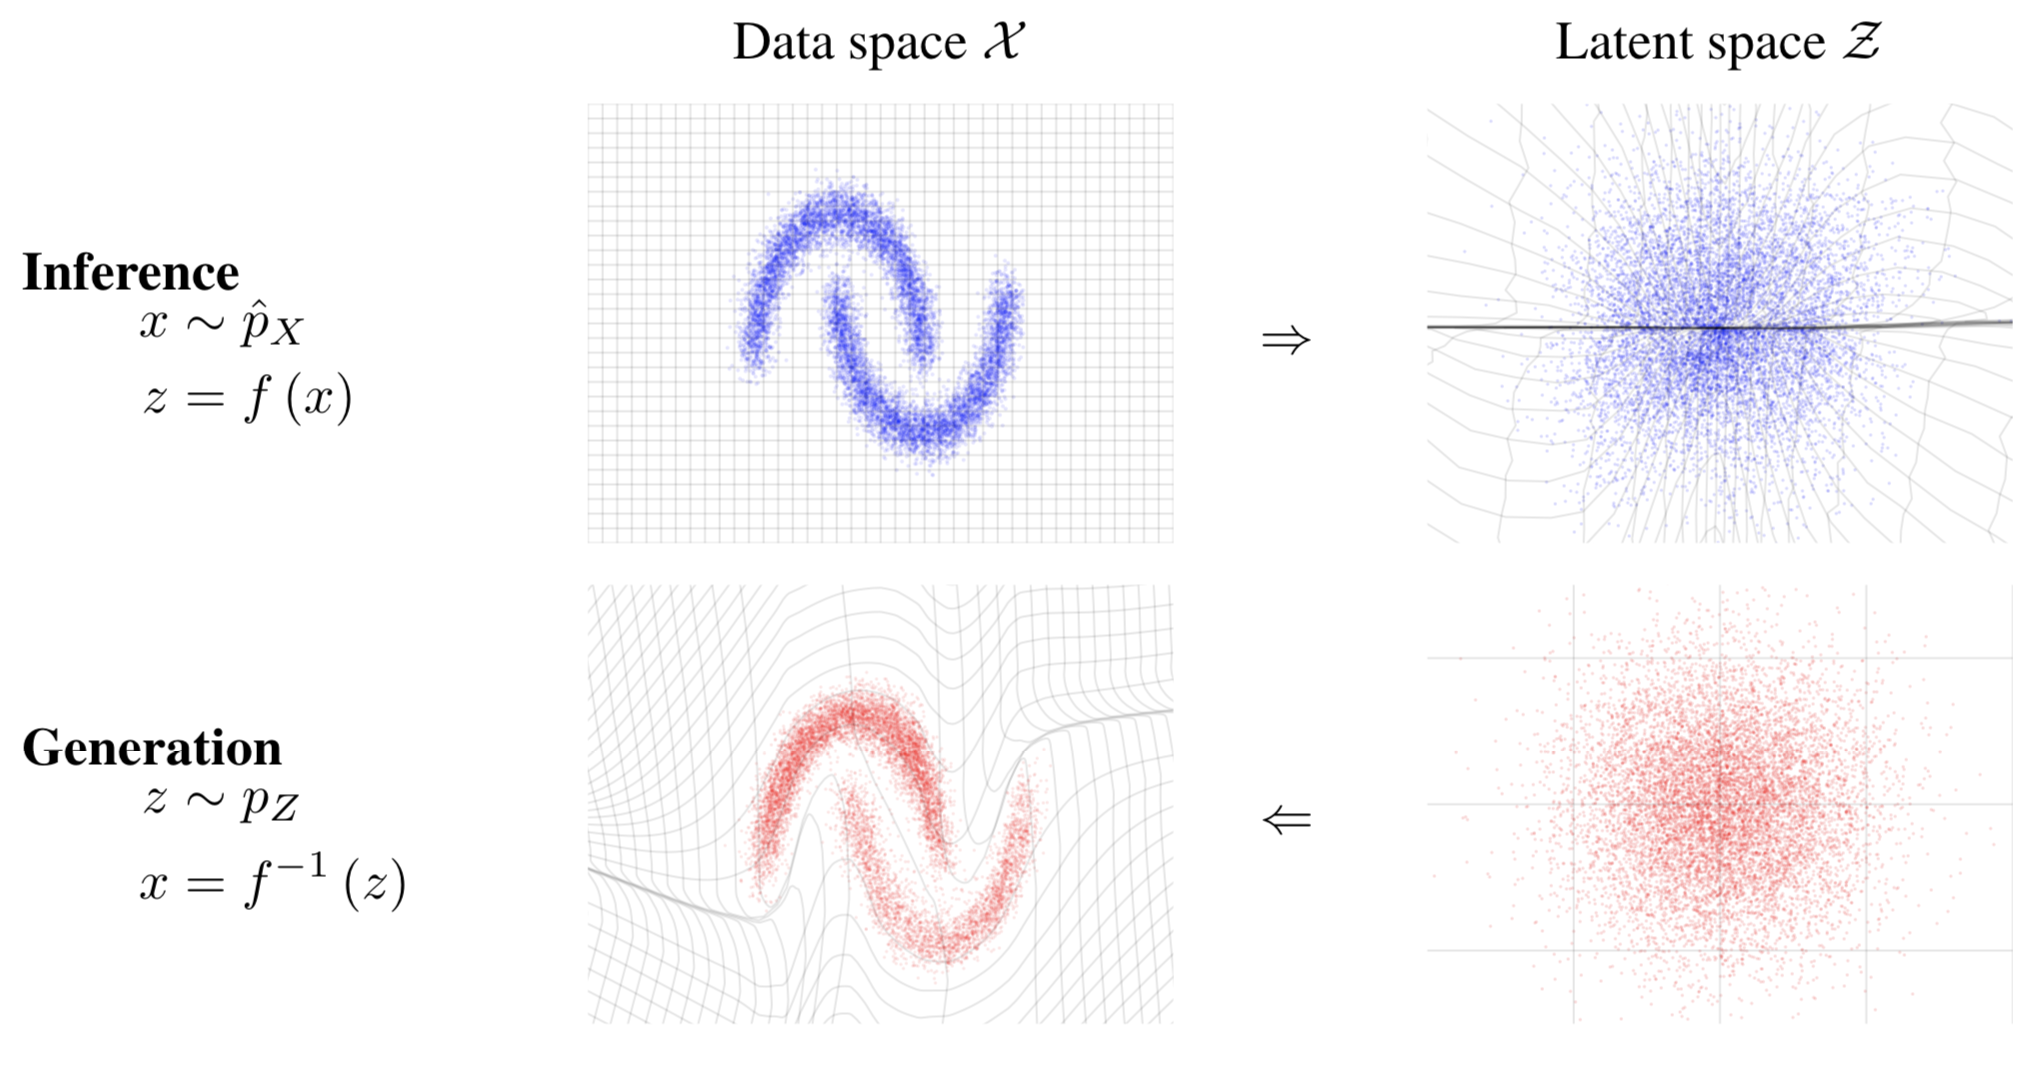
\includegraphics[width=0.85\linewidth]{figs/flows_how2}
	\end{figure}
	\vspace{-0.5cm}
	\begin{block}{Log likelihood}
		\vspace{-0.5cm}
		\[
			\log p(\bx | \btheta) = \log p(\bff_K \circ \dots \circ \bff_1(\bx)) + \sum_{k=1}^K\log |\det (\bJ_{\bff_k})|
		\]
	\end{block}
	\myfootnotewithlink{https://arxiv.org/abs/1605.08803}{Dinh L., Sohl-Dickstein J., Bengio S. Density estimation using Real NVP, 2016} 
\end{frame}
%=======
\begin{frame}{Recap of previous lecture}
	\vspace{-0.5cm}
	\begin{block}{Flow log-likelihood}
		\vspace{-0.3cm}
		\[
			\log p(\bx|\btheta) = \log p(\bff_{\btheta}(\bx)) + \log  |\det (\bJ_\bff)|
		\]
		\vspace{-0.5cm}
	\end{block}
	The main challenge is a determinant of the Jacobian.
	\begin{block}{Linear flows}	
		\vspace{-0.2cm}
		\[
			\bz = \bff_{\btheta}(\bx) = \bW \bx, \quad \bW \in \bbR^{m \times m}, \quad \btheta = \bW, \quad \bJ_\bff = \bW^T
		\]
	\end{block}
	\vspace{-0.3cm}
	\begin{itemize}
		\item LU-decomposition
		\[
			\bW = \mathbf{P} \bL \bU.
		\]
		\item QR-decomposition
		\[
			\bW = \bQ \mathbf{R}.
		\]
	\end{itemize}
	Decomposition should be done only once in the beggining. Next, we fit decomposed matrices ($\bP/\bL/\bU$ or $\bQ/\bR$).
	\myfootnote{\href{https://arxiv.org/abs/1807.03039}{Kingma D. P., Dhariwal P. Glow: Generative Flow with Invertible 1x1 Convolutions, 2018}  \\
	\href{https://arxiv.org/abs/1901.11137}{Hoogeboom E., et al. Emerging convolutions for generative normalizing flows, 2019}
	}
\end{frame}
%=======
\begin{frame}{Recap of previous lecture}
	Consider an autoregressive model
	\vspace{-0.3cm}
	{\small
		\[
		p(\bx | \btheta) = \prod_{j=1}^m p(x_j | \bx_{1:j - 1}, \btheta), \quad
		p(x_j | \bx_{1:j - 1}, \btheta) = \mathcal{N} \left(\mu_{j, \btheta}(\bx_{1:j-1}), \sigma^2_{j, \btheta} (\bx_{1:j-1})\right).
		\]
	}
	\vspace{-0.5cm}
	\begin{block}{Gaussian autoregressive NF}
		\vspace{-0.5cm}
		\begin{align*}
			\bx &= \bg_{\btheta}(\bz) \quad \Rightarrow \quad {\color{violet} x_j} = \sigma_{j, \btheta} ({\color{violet} \bx_{1:j-1}}) \cdot {\color{teal} z_j} + \mu_{j, \btheta}({\color{violet} \bx_{1:j-1}}). \\
			\bz &= \bff_{\btheta}(\bx) \quad \Rightarrow \quad {\color{teal} z_j} = \left({\color{violet}x_j} - \mu_{j, \btheta}({\color{violet}\bx_{1:j-1}}) \right) \cdot \frac{1}{ \sigma_{j, \btheta} ({\color{violet}\bx_{1:j-1}})}.
		\end{align*}
		\vspace{-0.5cm}
	\end{block}
	\begin{itemize}
		\item We have an \textbf{invertible} and \textbf{differentiable} transformation from $p(\bz)$ to $p(\bx | \btheta)$.
		\item Jacobian of such transformation is triangular!
	\end{itemize}
	Generation function $\bg_{\btheta}(\bz)$ is \textbf{sequential}. \\ Inference function $\bff_{\btheta}(\bx)$ is \textbf{not sequential}.
	
	\myfootnotewithlink{https://arxiv.org/abs/1705.07057}{Papamakarios G., Pavlakou T., Murray I. Masked Autoregressive Flow for Density Estimation, 2017} 
\end{frame}
%=======
\begin{frame}{Recap of previous lecture}
	Let split $\bx$ and $\bz$ in two parts: 
	\[
	\bx = [\bx_1, \bx_2] = [\bx_{1:d}, \bx_{d+1:m}]; \quad \bz = [\bz_1, \bz_2] = [\bz_{1:d}, \bz_{d+1:m}].
	\]
	\vspace{-0.5cm}
	\begin{block}{Coupling layer}
		\vspace{-0.5cm}
		\[
		\begin{cases} {\color{violet}\bx_1} = {\color{teal}\bz_1}; \\ {\color{violet}\bx_2} = {\color{teal}\bz_2} \odot \bsigma_{\btheta}({\color{teal}\bz_1}) + \bmu_{\btheta}({\color{teal}\bz_1}).\end{cases}  
		\begin{cases} {\color{teal}\bz_1} ={\color{violet} \bx_1}; \\ {\color{teal}\bz_2} = \left({\color{violet}\bx_2} - \bmu_{\btheta}({\color{violet}\bx_1}) \right) \odot \frac{1}{\bsigma_{\btheta}({\color{violet}\bx_1})}.\end{cases}
		\]
		Estimating the density takes 1 pass, sampling takes 1 pass!
	\end{block}
	\begin{block}{Jacobian}
		\vspace{-0.3cm}
		\[
		\det \left( \frac{\partial \bz}{\partial \bx} \right) = \det 
		\begin{pmatrix}
			\bI_d & 0_{d \times m - d} \\
			\frac{\partial \bz_2}{\partial \bx_1} & \frac{\partial \bz_2}{\partial \bx_2}
		\end{pmatrix} = \prod_{j=1}^{m - d} \frac{1}{\sigma_{j, \btheta}(\bx_1)}.
		\]
	\end{block}
	Coupling layer is a special case of autoregressive NF.
	
	\myfootnotewithlink{https://arxiv.org/abs/1605.08803}{Dinh L., Sohl-Dickstein J., Bengio S. Density estimation using Real NVP, 2016} 
\end{frame}
%=======
\begin{frame}{Outline}
    \tableofcontents
\end{frame}
%=======
\section{Forward and Reverse KL for NF}
%=======
\begin{frame}{Forward KL vs Reverse KL}
	\begin{block}{Forward KL $\equiv$ MLE}
		\vspace{-0.5cm}
		\begin{align*}
			KL(\pi || p) &= \int \pi (\bx) \log \frac{\pi(\bx)}{p(\bx | \btheta)} d \bx \\
			&= - \bbE_{\pi(\bx)} \log p(\bx | \btheta) + \text{const} \rightarrow \min_{\btheta}
		\end{align*}
	\end{block}
	\begin{block}{Forward KL for NF model}
	    \vspace{-0.1cm}
		\[
			\log p(\bx|\btheta) = \log p(\bff_{\btheta}(\bx)) + \log  |\det (\bJ_\bff)|
		\]		
		\[
			KL(\pi || p)  = - \bbE_{\pi(\bx)} \left[\log p(\bff_{\btheta}(\bx)) + \log  |\det (\bJ_\bff)|\right] + \text{const} 
		\]
		\vspace{-0.2cm}
		\begin{itemize}
			\item We need to be able to compute $\bff_{\btheta}(\bx)$ and its Jacobian.
			\item We need to be able to compute the density $p(\bz)$.
			\item We don’t need to think about computing the function $\bg_{\btheta}(\bz) = \bff^{-1}_{\btheta}(\bz)$ until we want to sample from the NF.
		\end{itemize}
	\end{block}
\end{frame}
%=======
\begin{frame}{Forward KL vs Reverse KL}
	\begin{block}{Reverse KL}
	  	\vspace{-0.5cm}
			\begin{align*}
				KL(p || \pi) &= \int p(\bx | \btheta) \log \frac{p(\bx | \btheta)}{\pi(\bx)} d \bx \\
				&= \bbE_{p(\bx | \btheta)} \left[{\color{violet}\log p(\bx | \btheta)} - \log \pi(\bx)\right] \rightarrow \min_{\btheta}
			\end{align*}
		\vspace{-0.7cm}
	\end{block}
	\begin{block}{Reverse KL for NF model (LOTUS trick)}
  		\vspace{-0.3cm}
		\[
			 \log p(\bx | \btheta) = \log p(\bz) +  \log  |\det (\bJ_\bff)| = \log p(\bz) - \log |\det (\bJ_\bg)| 
		\]
		\[
			KL(p || \pi)  = \bbE_{p(\bz)} \left[ {\color{violet} \log p(\bz) -  \log |\det (\bJ_\bg)| } - \log \pi(\bg_{\btheta}(\bz)) \right]
		\]
		\vspace{-0.3cm}
		\begin{itemize}
		\item We need to be able to compute $\bg_{\btheta}(\bz)$ and its Jacobian.
		\item We need to be able to sample from the density $p(\bz)$ (do not need to evaluate it) and to evaluate(!) $\pi(\bx)$.
		\item We don’t need to think about computing the function $\bff_{\btheta}(\bx)$.
		\end{itemize}
	\end{block}
\end{frame}
%=======
\begin{frame}{Normalizing flows KL duality}
	\begin{block}{Theorem}
		Fitting NF model $p(\bx| \btheta)$ to the target distribution $\pi(\bx)$ using forward KL (MLE) is equivalent to fitting the induced distribution $p(\bz| \btheta)$ to the base $p(\bz)$ using reverse KL:
		\vspace{-0.2cm}
		\[
			\argmin_{\btheta} KL(\pi(\bx) || p(\bx | \btheta)) = \argmin_{\btheta} KL(p(\bz | \btheta) || p(\bz)).
		\]
		\vspace{-0.7cm}
	\end{block}
	\begin{figure}
		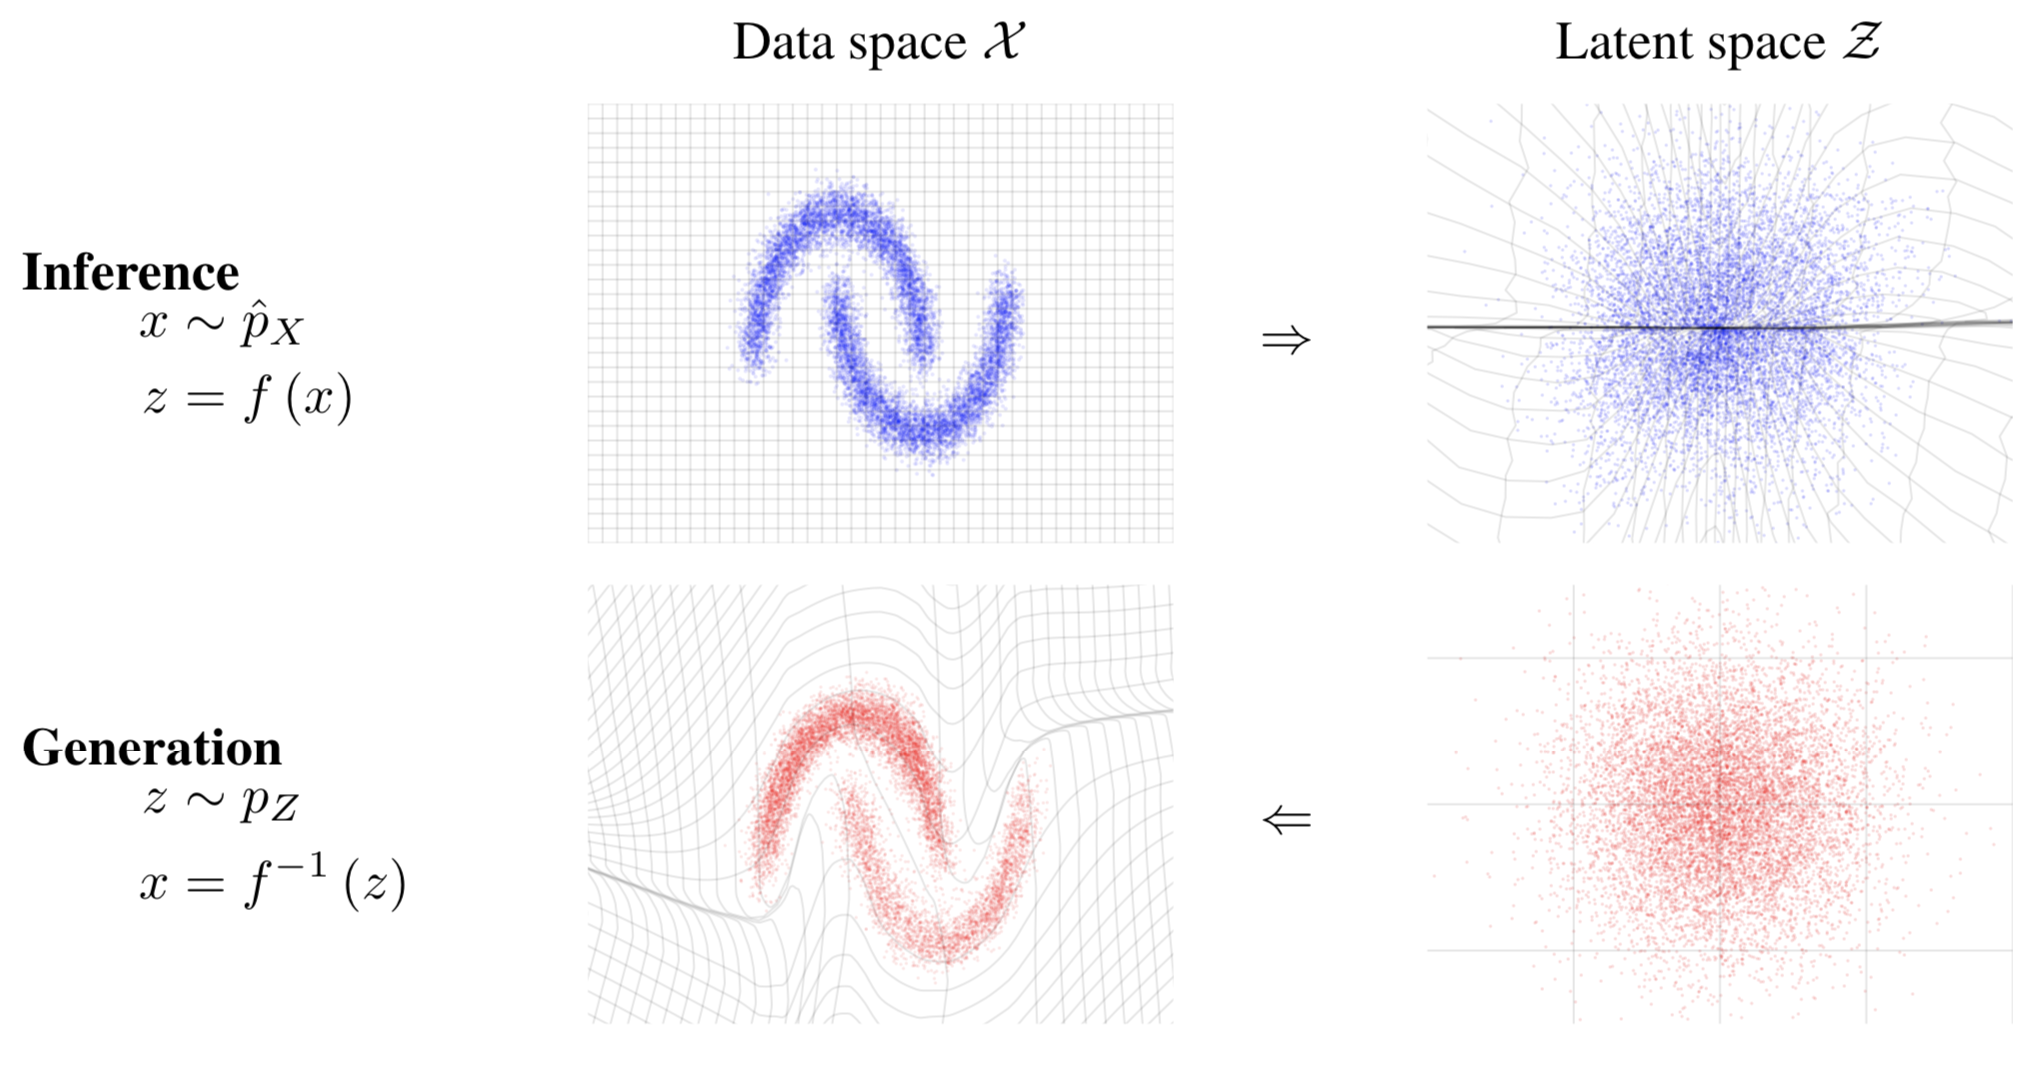
\includegraphics[width=0.85\linewidth]{figs/flows_how2}
	\end{figure}
	\myfootnotewithlink{https://arxiv.org/abs/1912.02762}{Papamakarios G. et al. Normalizing flows for probabilistic modeling and inference, 2019} 
\end{frame}
%=======
\begin{frame}{Normalizing flows KL duality}
	\begin{block}{Theorem}
		\vspace{-0.3cm}
		\[
			\argmin_{\btheta} KL(\pi(\bx) || p(\bx | \btheta)) = \argmin_{\btheta} KL(p(\bz | \btheta) || p(\bz)).
		\]
		\vspace{-0.5cm}
	\end{block}
	\begin{block}{Proof}
		\begin{itemize}
			\item $\bz \sim p(\bz)$, $\bx = \bg_{\btheta}(\bz)$, $\bx \sim p(\bx| \btheta)$;
			\item $\bx \sim \pi(\bx)$, $\bz = \bff_{\btheta}(\bx)$, $\bz \sim p(\bz | \btheta)$;
		\end{itemize}
		\vspace{-0.3cm}
		\begin{align*}
			\log p(\bz | \btheta) &= \log \pi(\bg_{\btheta}(\bz)) + \log | \det ( \bJ_\bg) |; \\
			\log p(\bx | \btheta) &= \log p(\bff_{\btheta}(\bx)) + \log | \det ( \bJ_\bff) |.
		\end{align*}
		\vspace{-0.9cm}
		\begin{multline*}
			KL\left(p(\bz | \btheta) || p(\bz) \right) = \mathbb{E}_{p(\bz | \btheta)} \bigl[ {\color{violet}\log p(\bz | \btheta)} - \log p(\bz) \bigr] = \\ 
			= \mathbb{E}_{{\color{olive}p(\bz | \btheta)}} \left[ {\color{violet}\log \pi(\bg_{\btheta}(\bz)) +  \log |\det (\bJ_\bg)|} - \log p(\bz) \right] = \\
			= \mathbb{E}_{{\color{olive}\pi(\bx)}} \left[ \log \pi(\bx) {\color{teal} - \log |\det (\bJ_\bff)| - \log p(\bff_{\btheta}(\bx))} \right] = \\
			= \mathbb{E}_{\pi(\bx)} \bigl[ \log \pi(\bx) {\color{teal} -\log p(\bx | \btheta)} \bigr] = KL (\pi(\bx) || p(\bx | \btheta)).
		\end{multline*}
	\end{block}
	\myfootnotewithlink{https://arxiv.org/abs/1705.07057}{Papamakarios G., Pavlakou T., Murray I. Masked Autoregressive Flow for Density Estimation, 2017} 
\end{frame}
%=======
\section{Latent variable models (LVM)}
%=======
\begin{frame}{Bayesian framework}
	\begin{block}{Bayes theorem}
		\vspace{-0.3cm}
		\[
			p(\btheta| \bx) = \frac{p(\bx | \btheta) p(\btheta)}{p(\bx)} = \frac{p(\bx | \btheta) p(\btheta)}{\int p(\bx | \btheta) p(\btheta) d \btheta} 
		\]
		\vspace{-0.3cm}
		\begin{itemize}
			\item $\bx$ -- observed variables, $\btheta$ -- unobserved variables (latent variables/parameters);
			\item $p(\bx | \btheta)$ -- likelihood;
			\item $p(\bx) = \int p(\bx | \btheta) p(\btheta) d \btheta$ -- evidence;
			\item $p(\btheta)$ -- prior distribution, $p(\btheta| \bx)$ -- posterior distribution.
		\end{itemize}
	\end{block}
	\begin{block}{Meaning}
		\begin{itemize}
			\item We have unobserved variables $\btheta$ and some prior knowledge about them $p(\btheta)$.
			\item Then, the data $\bx$ has been observed. 
			\item Posterior distribution $p(\btheta| \bx)$ summarizes the knowledge after the observations $\bx$.
		\end{itemize} 
	\end{block}
\end{frame}
%=======
\begin{frame}{Bayesian framework}
	Let consider the case, where the unobserved variables $\btheta$ are the model parameters (we treat model parameters $\btheta$ as random variables).
	\begin{itemize}
		\item $\bX = \{\bx_i\}_{i=1}^n$ -- observed samples;
		\item $p(\btheta)$ -- prior distribution.
	\end{itemize}
	\begin{block}{Posterior distribution}
		\[
			p(\btheta | \bX) = \frac{p(\bX | \btheta) p(\btheta)}{p(\bX)} = \frac{p(\bX | \btheta) p(\btheta)}{\int p(\bX | \btheta) p(\btheta) d \btheta} 
		\]
		\vspace{-0.2cm}
	\end{block}
	If evidence $p(\bX)$ is intractable (due to multidimensional integration), we can't get posterior distribution.
    \begin{block}{Maximum a posteriori (MAP) estimation}
	    \vspace{-0.2cm}
	    \[
	        \btheta^* = \argmax_{\btheta} p(\btheta | \bX) = \argmax_{\btheta} \bigl(\log p(\bX | \btheta) + \log p(\btheta) \bigr)
	    \]
    \end{block}
\end{frame}
%=======
\begin{frame}{Latent variable models (LVM)}
	\begin{block}{MLE problem}
		\vspace{-0.5cm}
		\[
		\btheta^* = \argmax_{\btheta} p(\bX | \btheta) = \argmax_{\btheta} \prod_{i=1}^n p(\bx_i | \btheta) = \argmax_{\btheta} \sum_{i=1}^n \log p(\bx_i | \btheta).
		\]
		\vspace{-0.5cm}
	\end{block}
	The distribution $p(\bx | \btheta)$ could be complicated and intractable (as well as real distribution $\pi(\bx)$).
	\begin{block}{Extended probabilistic model}
		Introduce latent variable $\bz$ for each sample $\bx$
		\[
		p(\bx, \bz | \btheta) = p(\bx | \bz, \btheta) p(\bz); \quad 
		\log p(\bx, \bz | \btheta) = \log p(\bx | \bz, \btheta) + \log p(\bz).
		\]
		\[
		p(\bx | \btheta) = \int p(\bx, \bz | \btheta) d\bz = \int p(\bx | \bz, \btheta) p(\bz) d\bz.
		\]
	\end{block}
	\vspace{-0.3cm}
	\begin{block}{Motivation}
		The distributions $p(\bx | \bz, \btheta)$ and $p(\bz)$ could be quite simple.
	\end{block}
\end{frame}
%=======
\begin{frame}{Latent variable models (LVM)}
	\[
	\log p(\bx | \btheta) = \log \int p(\bx | \bz, \btheta) p(\bz) d\bz \rightarrow \max_{\btheta}
	\]
	\vspace{-0.6cm}
	\begin{block}{Examples}
		\begin{minipage}[t]{0.45\columnwidth}
			\textit{Mixture of gaussians} \\
			\vspace{-0.5cm}
			\begin{figure}
				\centering
				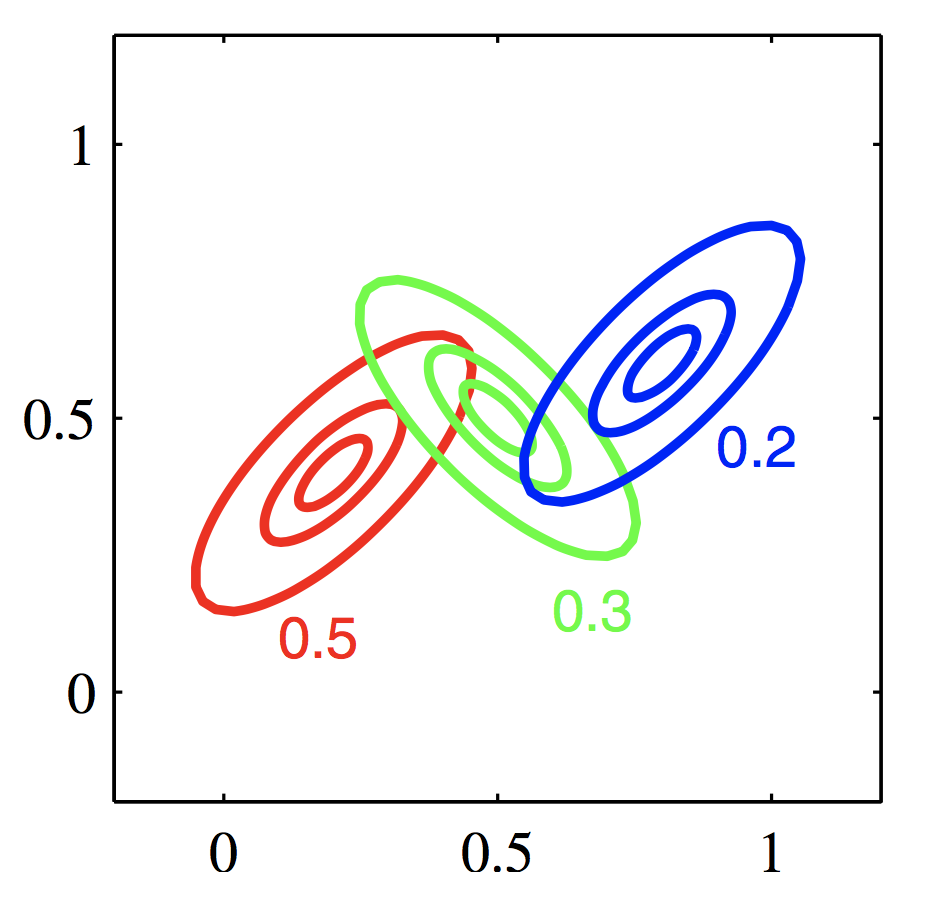
\includegraphics[width=0.75\linewidth]{figs/mixture_of_gaussians}
			\end{figure}
			\vspace{-0.5cm}
			\begin{itemize}
				\item $p(\bx | z, \btheta) = \cN(\bmu_z, \bSigma_z)$
				\item $p(z) = \text{Categorical}(\bpi)$
			\end{itemize}
		\end{minipage}%
		\begin{minipage}[t]{0.53\columnwidth}
			\textit{PCA model} \\
			\vspace{-0.5cm}
			\begin{figure}
				\centering
				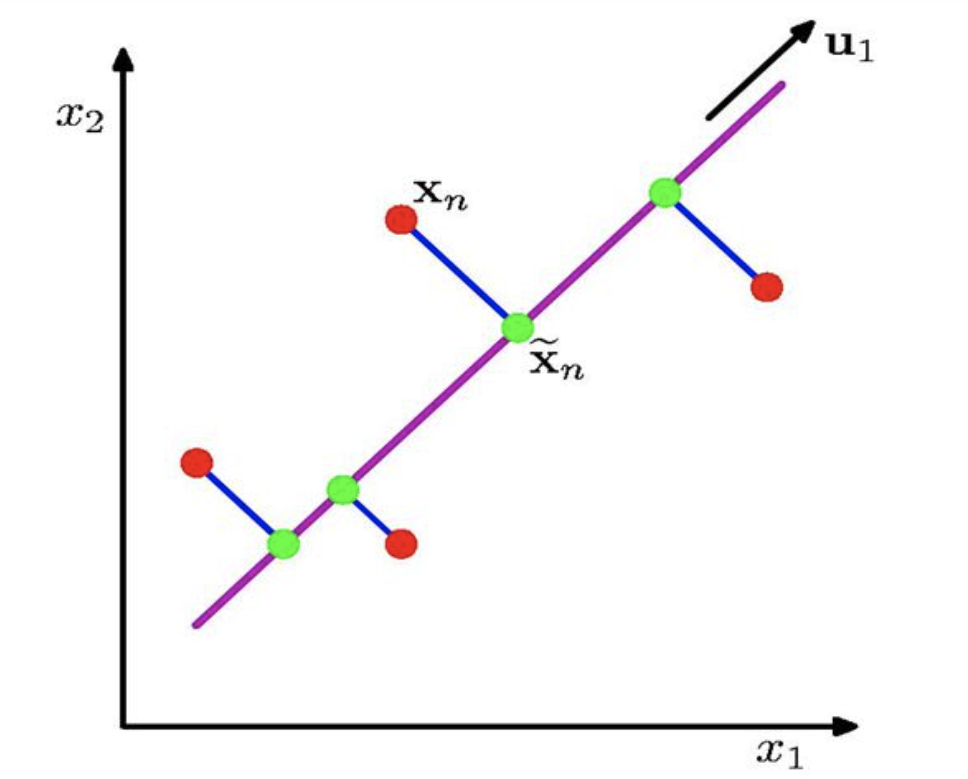
\includegraphics[width=.7\linewidth]{figs/pca}
			\end{figure}
			\vspace{-0.3cm}
			\begin{itemize}
				\item $p(\bx | \bz, \btheta) = \cN(\bW \bz + \bmu, \sigma^2 \bI)$
				\item $p(\bz) = \cN(0, \bI)$
			\end{itemize}
		\end{minipage}
	\end{block}
	\myfootnote{Bishop\,C. Pattern Recognition and Machine Learning, 2006}
\end{frame}
%=======
\begin{frame}{MLE for LVM}
	\vspace{-0.3cm}
	\[
		\sum_{i=1}^n \log p(\bx_i | \btheta) = \sum_{i=1}^n \log \int p(\bx_i| \bz_i, \btheta) p(\bz_i) d\bz_i \rightarrow \max_{\btheta}.
	\]
	\vspace{-0.3cm}
	\begin{figure}
		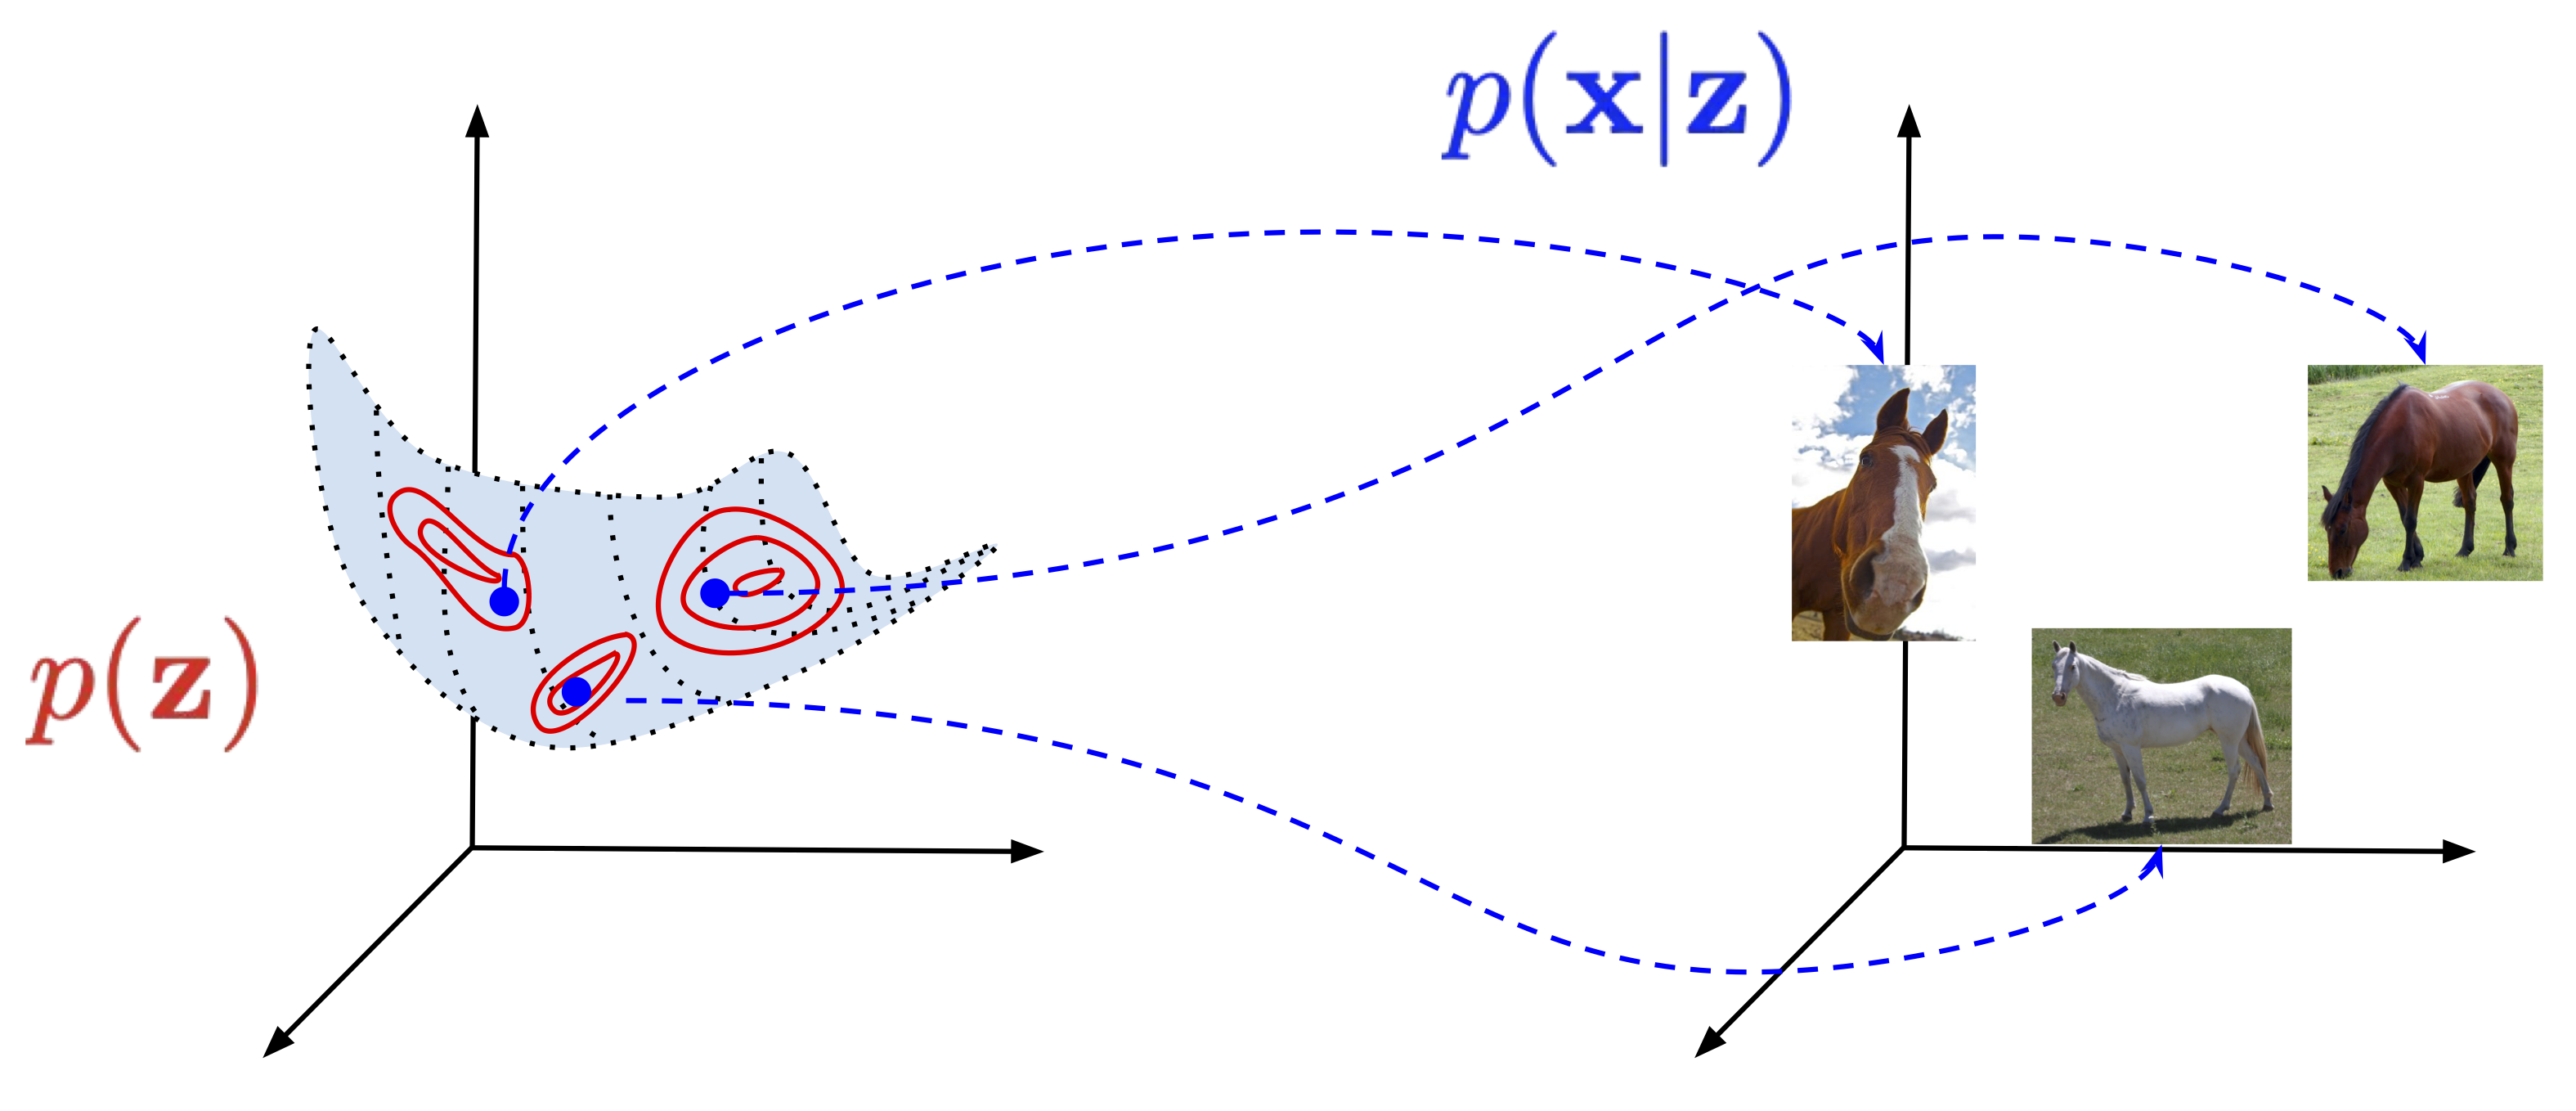
\includegraphics[width=.65\linewidth]{figs/lvm_diagram}
	\end{figure}
	\vspace{-0.3cm}
	\begin{block}{Naive approach}
		\vspace{-0.7cm}
		\[
			p(\bx | \btheta) = \int p(\bx | \bz, \btheta) p(\bz) d\bz = \bbE_{p(\bz)} p(\bx | \bz, \btheta) \approx \frac{1}{K} \sum_{k=1}^{K} p(\bx | \bz_k, \btheta),
		\]
		\vspace{-0.5cm} \\
		where $\bz_k \sim p(\bz)$. \\
		\textbf{Challenge:} to cover the space properly, the number of samples grows exponentially with respect to dimensionality of $\bz$. 
	\end{block}
	\myfootnotewithlink{https://jmtomczak.github.io/blog/4/4\_VAE.html}{image credit: https://jmtomczak.github.io/blog/4/4\_VAE.html}
\end{frame}
%=======
\section{Variational lower bound (ELBO)}
%=======
\begin{frame}{ELBO derivation I}
	\begin{block}{Inequality derivation}
		\vspace{-0.7cm}
		\begin{multline*}
			\log p(\bx| \btheta) 
			= \log \int p(\bx, \bz | \btheta) d\bz = \log \int \frac{q(\bz)}{q(\bz)} p(\bx, \bz | \btheta) d\bz = \\
			= \log \bbE_{q} \left[\frac{p(\bx, \bz| \btheta)}{q(\bz)} \right] \geq \bbE_{q} \log \frac{p(\bx, \bz| \btheta)}{q(\bz)} = \cL_{q, \btheta}(\bx)
		\end{multline*}
		\vspace{-0.3cm}
	\end{block}
	Here $q(\bz)$ is an arbitrary distribution ($\int q(\bz) d\bz = 1$).
	\begin{block}{Variational lower bound (ELBO)}
		\[
			 \cL_{q, \btheta}(\bx) = \bbE_{q} \log \frac{p(\bx, \bz| \btheta)}{q(\bz)}  \leq \log p(\bx| \btheta) 
		\]
		This inequality holds for every distribution $q(\bz)$.
	\end{block}
\end{frame}
%=======
\begin{frame}{ELBO derivation II}
	\vspace{-0.3cm}
	\[
		{\color{teal}p(\bz|\bx, \btheta) = \frac{p(\bx, \bz | \btheta)}{p(\bx| \btheta)}}
	\]
	\vspace{-0.4cm}
	\begin{block}{Equality derivation}
		\vspace{-0.7cm}
		\begin{multline*}
			\cL_{q, \btheta}(\bx) = \int q(\bz) \log \frac{\color{teal}p(\bx, \bz | \btheta)}{q(\bz)}d\bz = \\ 
			= \int q(\bz) \log \frac{\color{teal}p(\bz|\bx, \btheta)p(\bx| \btheta)}{q(\bz)}d\bz = \\
			= \int q(\bz) \log p(\bx| \btheta) d\bz + \int q(\bz) \log \frac{p(\bz|\bx, \btheta)}{q(\bz)}d\bz = \\
			= \log p(\bx| \btheta) - KL(q(\bz) || p(\bz|\bx, \btheta))
		\end{multline*}
	\end{block}
	\vspace{-0.7cm}
	\begin{block}{Variational decomposition}
		\vspace{-0.2cm}
		\[
			\log p(\bx| \btheta) = \cL_{q, \btheta}(\bx) + {\color{violet}KL(q(\bz) || p(\bz|\bx, \btheta))} \geq \cL_{q, \btheta}(\bx).
		\]
	\end{block}
	Here ${\color{violet}KL(q(\bz) || p(\bz|\bx, \btheta)) \geq 0}$.
\end{frame}
%=======
\begin{frame}{Variational lower bound (ELBO)}
	\vspace{-0.3cm}
	\begin{align*}
		\cL_{q, \btheta}(\bx) &= \int q(\bz) \log \frac{\color{violet}p(\bx, \bz | \btheta)}{\color{teal}q(\bz)}d\bz = \\ 
		&= \int q(\bz) \log {\color{violet}p(\bx | \bz, \btheta)} d\bz + \int q(\bz) \log \frac{\color{violet}p(\bz)}{\color{teal}q(\bz)}d\bz \\ 
		&= \mathbb{E}_{q} \log p(\bx | \bz, \btheta) - KL (q(\bz) || p(\bz))
	\end{align*}
	\vspace{-0.5cm}
	\begin{block}{Log-likelihood decomposition}
		\vspace{-0.8cm}
		\begin{multline*}
			\log p(\bx| \btheta) = {\color{olive}\cL_{q, \btheta}(\bx)} + KL(q(\bz) || p(\bz|\bx, \btheta)) \\ = {\color{olive}\mathbb{E}_{q} \log p(\bx | \bz, \btheta) - KL (q(\bz) || p(\bz))} + KL(q(\bz) || p(\bz|\bx, \btheta)).
		\end{multline*}
		\vspace{-0.7cm}
	\end{block}
	\begin{itemize}
		\item Instead of maximizing incomplete likelihood, maximize ELBO
		\[
		\max_{\btheta} p(\bx | \btheta) \quad \rightarrow \quad \max_{q, \btheta} \cL_{q, \btheta}(\bx)
		\]
		\item Maximization of ELBO by \textbf{variational} distribution $q$ is equivalent to minimization of KL
		\[
		\argmax_q \cL_{q, \btheta}(\bx) \equiv \argmin_q KL(q(\bz) || p(\bz|\bx, \btheta)).
		\]
	\end{itemize}
\end{frame}
%=======
\section{EM-algorithm}
%=======
\begin{frame}{EM-algorithm}
	\vspace{-0.5cm}
	\begin{multline*}
		\cL_{q, \btheta}(\bx)  =  \mathbb{E}_{q} \log p(\bx | \bz, \btheta) - KL (q(\bz) || p(\bz)) = \\ = \bbE_q \left[ \log p(\bx | \bz, \btheta) - \log \frac{q(\bz)}{p(\bz)} \right]d\bz \rightarrow \max_{q, \btheta}.
	\end{multline*}
	\vspace{-0.5cm}
	\begin{block}{Block-coordinate optimization}
		\begin{itemize}
			\item Initialize $\btheta^*$;
			\item \textbf{E-step} ($\cL_{q, \btheta}(\bx) \rightarrow \max_q$)
			\vspace{-0.2cm}
			\begin{multline*}
				q^*(\bz) = \argmax_q \cL_{q, \btheta^*}(\bx) = \\
				= \argmin_q KL(q(\bz) || p(\bz | \bx, \btheta^*)) = p(\bz| \bx, \btheta^*);
			\end{multline*}
			\item \textbf{M-step} ($\cL_{q, \btheta}(\bx) \rightarrow \max_{\btheta}$)
			\vspace{-0.2cm}
			\[
			\btheta^* = \argmax_{\btheta} \cL_{q^*, \btheta}(\bx);
			\]
			\vspace{-0.2cm}
			\item Repeat E-step and M-step until convergence.
		\end{itemize}
	\end{block}
\end{frame}
%=======
\begin{frame}{EM-algorithm illustration}
	\begin{minipage}[t]{0.45\columnwidth}
		\begin{figure}
			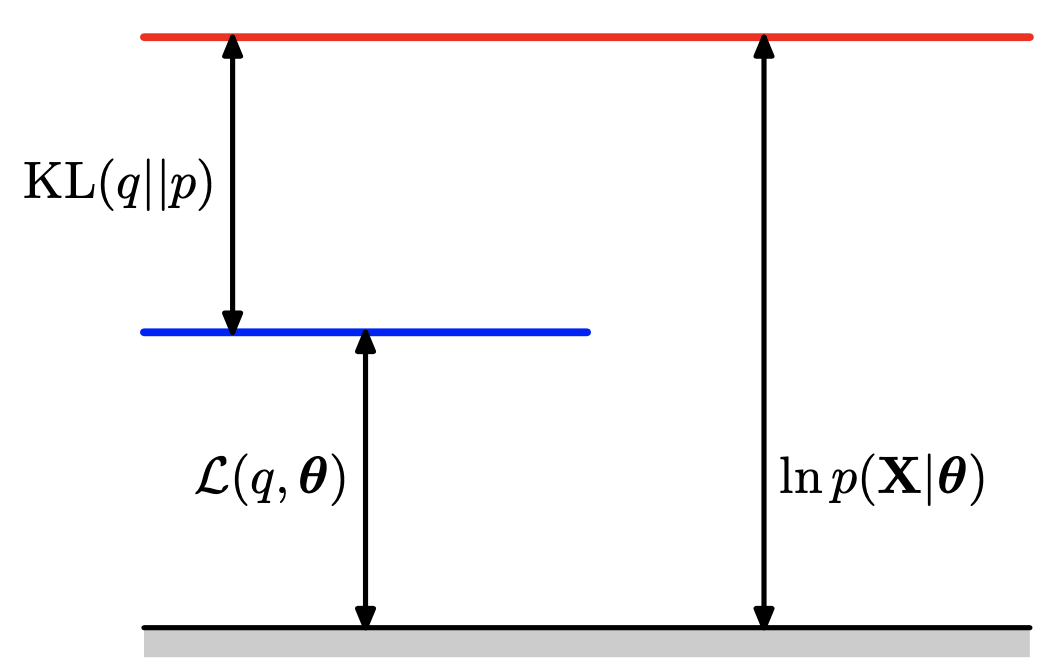
\includegraphics[width=0.9\linewidth]{figs/em_bishop1}
		\end{figure}
	\end{minipage}%
	\begin{minipage}[t]{0.55\columnwidth}
		\begin{figure}
			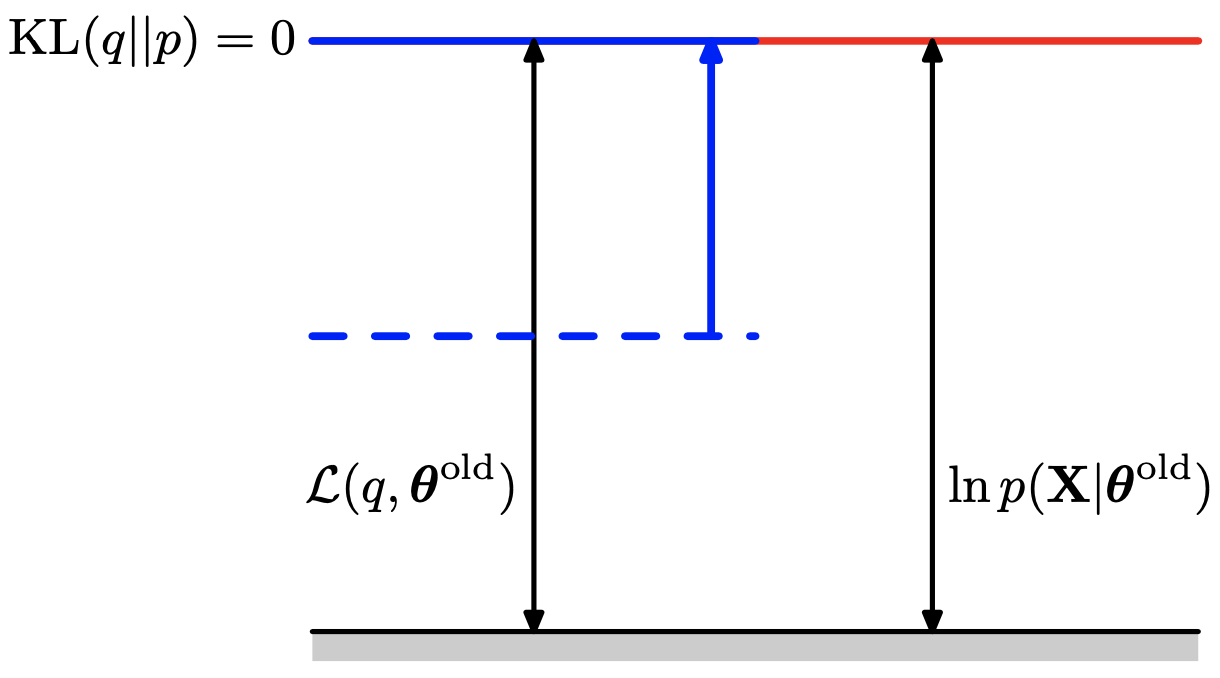
\includegraphics[width=0.85\linewidth]{figs/em_bishop2}
		\end{figure}
	\end{minipage}
	\begin{figure}
		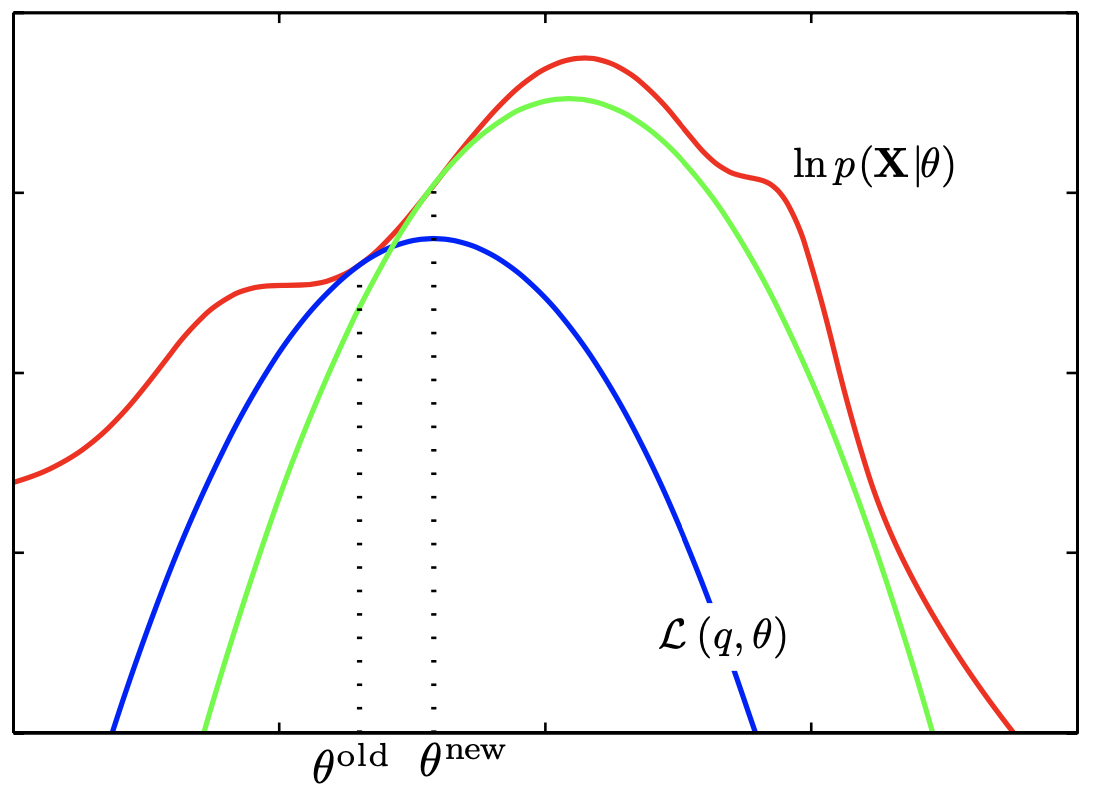
\includegraphics[width=.55\linewidth]{figs/em_bishop3}
	\end{figure}
	
	\myfootnote{Bishop\,C. Pattern Recognition and Machine Learning, 2006}
\end{frame}
%=======
\begin{frame}{Summary}
	\begin{itemize}
		\item Flow duality connects data space and latent space via forward and reverse KL formulations. 
		\vfill
		\item Bayesian framework is a generalization of most common machine learning tasks.
		\vfill
		\item LVM introduces latent representation of observed samples to make model more interpretative.
		\vfill
		\item LVM maximizes variational evidence lower bound (ELBO) to find MLE for the parameters.
		\vfill
		\item The general variational EM algorithm maximizes ELBO objective for LVM model to find MLE for parameters $\btheta$.	
	\end{itemize}
\end{frame}
\end{document} 